
In the following section, I describe the agriculture industry in Scotland; beaver ecology, tendencies in territorial expansion, and behavior, including potential threats to agricultural productivity; and the Scotland's history of beaver extermination and recent reemergence. 

\subsection{Agriculture in Scotland}

In 2023, 69\% (5.33 million hectares) of Scotland's land area was devoted to agricultural use \citep{cabinet_secretary_for_rural_affairs_land_reform_and_islands_results_2023}, with much of the arable farming concentrated along the eastern lowlands. The industry employs a 66,000-person workforce (about 1.2\% of the country's population), contributing approximately 2.5 billion euros of Standard Output.\footnote{A standard EU metric for measuring the economic weight of agricultural activity, standard output equals the average value of output (in euros) per hectare of farmland or per head of livestock.}

Most arable farming is dedicated to above-ground cereals, including barley, oats, and rye, and to a lesser extent, crops such as oilseed rape and beans.

[Are most farmers small or large]

Modern Scottish agriculture, built in a cool and marshy environment, has relied on an array of floodbanks constructed along rivers to protect cropland from inundation (CITE).

\begin{itemize}
    \item Ag output and employment (ie, communicate the scale of economic importance to the country and more broadly to the region), and put it in relative terms to rest of the UK/proportion of UK output
    \item Main crop types and land uses (put a map of land use in Scotland around here. Mention Tayside as a valuable lowland arable area, in contrast to the rugged highlands which are primarily used for herding)
\end{itemize}

\subsection{Beavers}

\begin{itemize}
    \item Habitat: Where do they live? What kinds of environmental variables influence their habitation \parencite{swinnen_environmental_2019}?
    \item Ecosystem engineers: Dam, burrow, and lodge construction
    \begin{itemize}
        \item Ecosystem service benefits citations here.
    \end{itemize}
    \item Familial structures $\rightarrow$ dispersion patterns
    \item Behavior: potential costs to agricultural productivity
    \begin{itemize}
        \item Burrowing $\rightarrow$ collapsing fields, floodbanks
        \item Dam building $\rightarrow$ backing up rivers and flooding fields
        \item Crop grazing
        \item Timber felling
    \end{itemize}
\end{itemize}

\subsection{Beavers in Scotland}

\begin{itemize}
    \item Extinction by pelt hunting
    \item Beaver reintroductions in eastern Europe, moving west
    \item Debate over introduction in the 1990s, followed by sanctuaries (Ramsey estate) and Knapdale controlled reintroduction (2009)
    \item Unauthorized emergence in the 2000s, across Tay, Earn, South Esk, Lunan, and Perth Coastal catchments (\cite{noauthor_beavers_2017}). See Fig. \ref{fig:study-area}. 
\end{itemize}

\begin{figure}
    \centering
    \caption{Study region}
    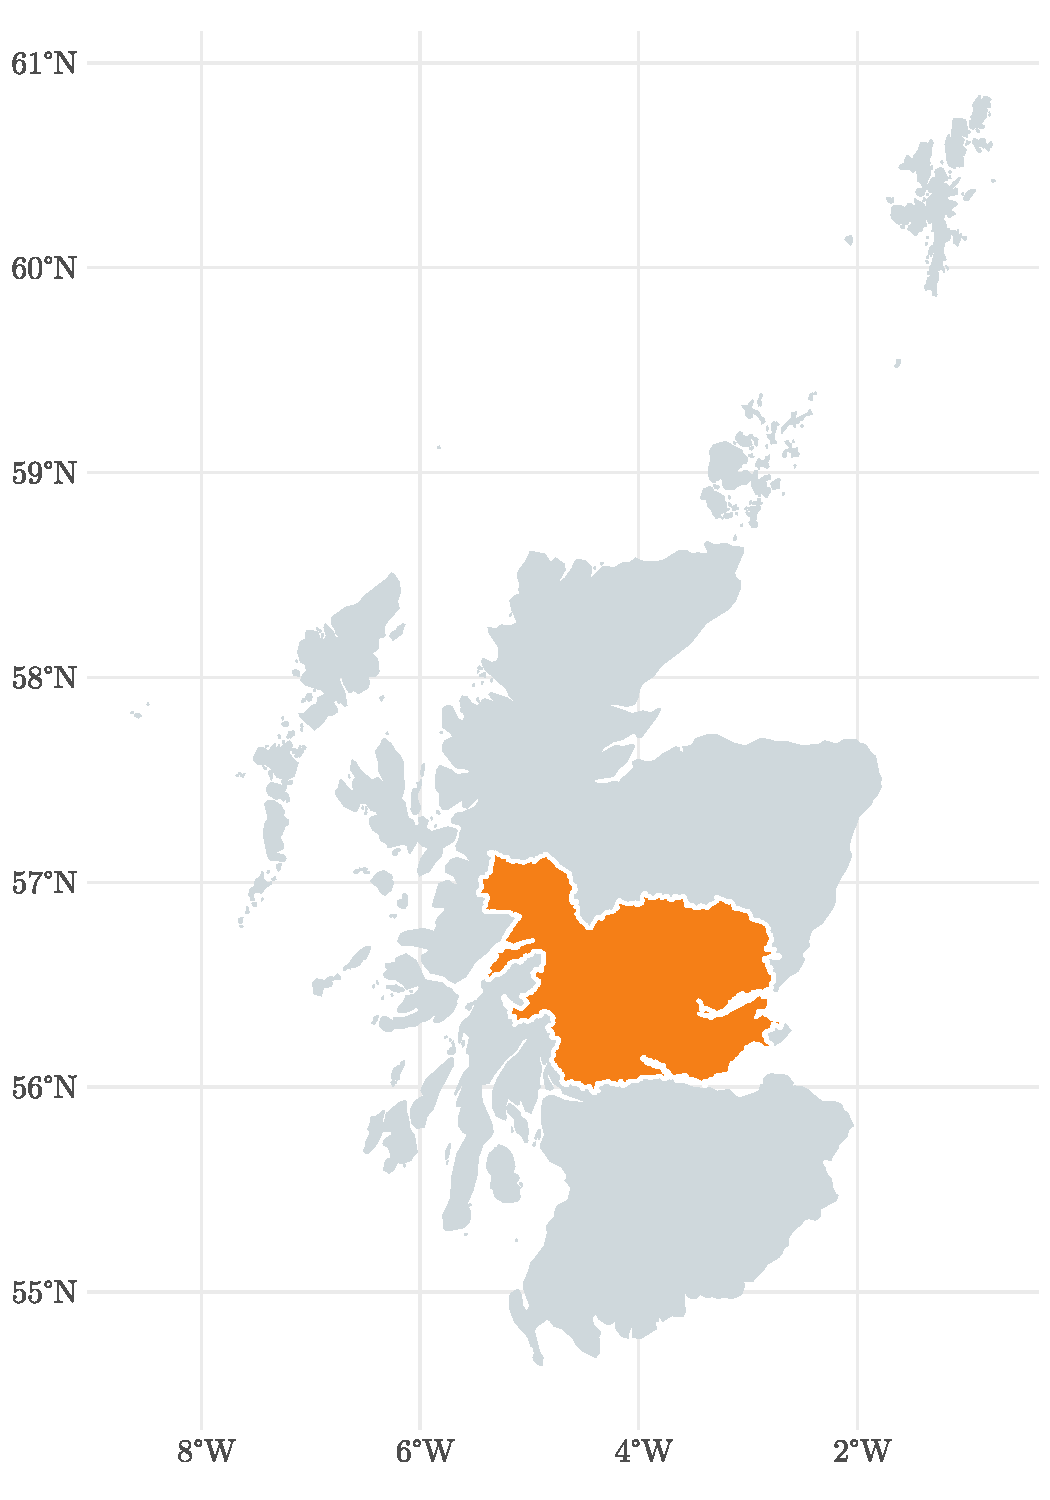
\includegraphics[width=0.5\linewidth]{output/figures/study_area.pdf}
    \label{fig:study-area}
    \caption*{\justifying \footnotesize Notes: Study region, capturing the area of beaver expansion around the Tay, Earn, South Esk, Lunan, and Perth Coastal catchments, is highlighted in orange within Scotland. Agricultural parish boundaries are drawn in gray.}
\end{figure}